\documentclass{beamer}
\usetheme{default}

\title{The Hopf fibration}
\author{Martin de Borbon}

\usepackage{amsmath, amsthm, amssymb}
\usepackage{graphicx}
\usepackage{tikz}

\newcommand{\R}{\mathbb{R}}
\newcommand{\C}{\mathbb{C}}
\newcommand{\CP}{\mathbb{CP}}
\newcommand{\va}{\vec{a}}
\newcommand{\vb}{\vec{b}}
\newcommand{\vu}{\vec{u}}
\newcommand{\vp}{\vec{p}}

\begin{document}
\begin{frame}[plain]
    \maketitle
\end{frame}

\begin{frame}{The Hopf map}
	\pause
	The \(n\)-dimensional sphere \(S^n\) is the set of points \((x_0, \ldots, x_n)\) in \(\R^{n+1}\) such that
	\[
	x_0^2 + \ldots + x_n^2 = 1 
	\]
	\pause
	The Hopf map \(H: S^3 \to S^2\) is given by
	\begin{equation*}
		H(a, b, c, d) = (a^2 + b^2 - c^2 - d^2, 2(ac + bd), 2(bc-ad) ) 
	\end{equation*}
	\pause
	We will discuss this map from two points of view
	\begin{itemize}
		\pause
		\item The group of rotations \(SO(3)\)
		\pause
		\item Complex lines in \(\C^2\)
	\end{itemize}
\end{frame}

\begin{frame}{Translations}
	\begin{itemize}
		\pause
		\vfill\item MAA250: \emph{A vector is quantity that has both direction and magnitude.}
		\pause
		\vfill\item Composition of two translations:
		\begin{figure}
			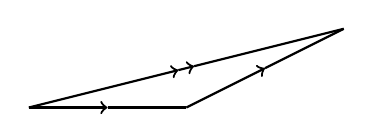
\begin{tikzpicture}
			\draw[->, thick] (0,0) -> (1,0);
			\draw[thick] (1, 0) -- (2,0);
			\draw[->, thick] (2,0) -- (3,.5);
			\draw[thick] (3, .5) -- (4,1);
			\draw[->, thick] (0,0) -- (1.9,.475);
			\draw[->, thick] (1.9, .475) -- (2.1, .525);
			\draw[thick] (2.1, .525) -- (4,1);
			\end{tikzpicture}
		\end{figure}
		\pause
		\vfill\item \textbf{Question:} Can we do something similar for rotations?
	\end{itemize}
\end{frame}

\begin{frame}{Rotations}
	\begin{itemize}
		\pause
		\item A rotation about the origin in \(\R^3\) can be specified by giving a
		vector for the axis and an angle
		\pause
		\item \textbf{Remark:} Rotations do not commute
		\pause
		\item Composition of two rotations:
		\begin{figure}
			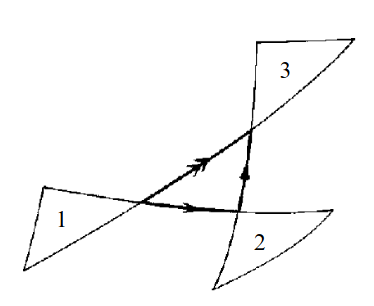
\includegraphics[scale=.4]{rotations.png}
			\caption{The segments are great circle arcs, each representing a rotation through twice the angle measured by the arc.}
		\end{figure}
	\end{itemize}
\end{frame}

\begin{frame}{Quaternions}
	\begin{itemize}
		\pause
		\item Mathematical vandalism (1843): Sir William Hamilton craved with his penknife into the side of Broom Bridge
		\[
		i^2 = j^2 = k^2 = ijk = -1
		\]
		also \(ij = -ji = k\) and cyclic permutations
		\pause
		\item A quaternion is an element of the form 
		\[
		a = a_0 + \underbrace{a_1 i + a_2 j + a_3 k}_{\va}
		\]
		where \(a_0, a_1, a_2, a_3 \in \R\)
		\pause
		\item The multiplication rules for \(i, j, k\) define the product
		\[
		a b = \underbrace{a_0 b_0 - \va \cdot \vb}_{\text{scalar}} + \underbrace{a_0 \vb + b_0 \va + \va \times \vb}_{\text{vector}}
		\]
	\end{itemize}
\end{frame}

\begin{frame}{Properties}
	The quaternions form an associative normed division algebra 
	\begin{itemize}
		\pause
		\item Associative: left and right multiplication commute
		\[
		(ab)c = a(bc)
		\]
		\pause
		\item The squared norm of \(a\) is
		\[
		|a|^2 = a a^* = a^* a = a_0^2 + a_1^2 + a_2^2 + a_3^2 
		\]
		where \(a^* = a_0 - \va\) is its conjugate. Key property:
		\[
		| ab | = |a| |b|
		\] 
		\pause
		\item Division: if \(a \neq 0\) then
		\[
		a^{-1} = \frac{a^*}{|a|^2}
		\]
	\end{itemize}	
\end{frame}

\begin{frame}{Unit quaternions acting by rotations}
	A unit quaternion \(u = \cos \theta + \sin \theta \vu \) defines \(R_u \in SO(3)\) given by
	\[
	R_u (\vp) = u \vp u^{-1}
	\]
	\begin{itemize}
		\pause
		\item \(R_u\) is a rotation about \(\vu\) by an angle \(2 \theta\)
		\pause
		\item \textbf{Example:} \(R_i, R_j, R_k\) are \(180^{\circ}\) rotations about the \(x, y, z\) axis
	\end{itemize}
	\pause
	Fix \(\vec{N} = (0,0,1)\) in \(S^2\). The Hopf map \(H:S^3 \to S^2\) is
	\[
	H(u) = R_u(\vec{N})
	\]
	\pause
	The pre-image of \(\vec{N}\) is a circle of unit quaternions acting by rotations about the \(z\)-axis. Other fibres are conjugate to this circle.
\end{frame}

\begin{frame}{Spinors}
	The assignment \(u \mapsto R_u\) is a group homomorphism
	\[
	Spin(3) \cong S^3 \xrightarrow{2:1} SO(3)
	\]	
	\begin{figure}
		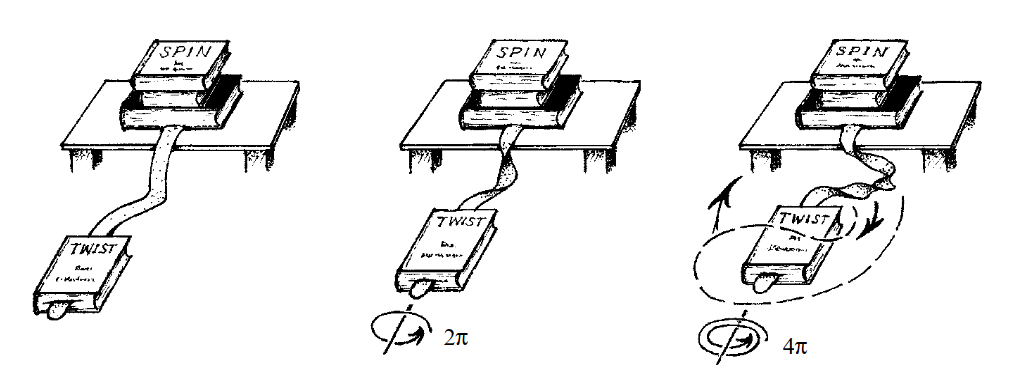
\includegraphics[scale=.3]{spin.png}
		\caption{A spinor turns into its negative after a complete rotation by \(360^{\circ}\)}
	\end{figure}
\end{frame}

\begin{frame}{Complex projective space}
	\(\CP^n\) is the space of complex lines going through the origin in \(\C^{n+1}\)
	\[
	\CP^n = \big( \C^{n+1} \setminus \{0\} \big) \, \big/ \, \C^*
	\]
	Points of \(\CP^n\) are equivalence classes
	\[
	[z_0, \ldots, z_n] = [\lambda z_0, \ldots, \lambda z_n] 
	\]
	\begin{itemize}
		\pause
		\item Restrict the quotient map to the unit sphere we obtain
		\[
		H: S^{2n+1} \to \CP^n
		\]
		\pause
		\item \(\CP^1\) is obtained from \(2\) copies of \(\C\) glued by
		\[
		\xi \mapsto 1/\xi
		\]
	\end{itemize}
\end{frame}

\begin{frame}{Stereographic projection}
	Projections from antipodal points are related by inversion in the unit sphere \(S^{n-1} \subset \R^n\)
	\begin{figure}
		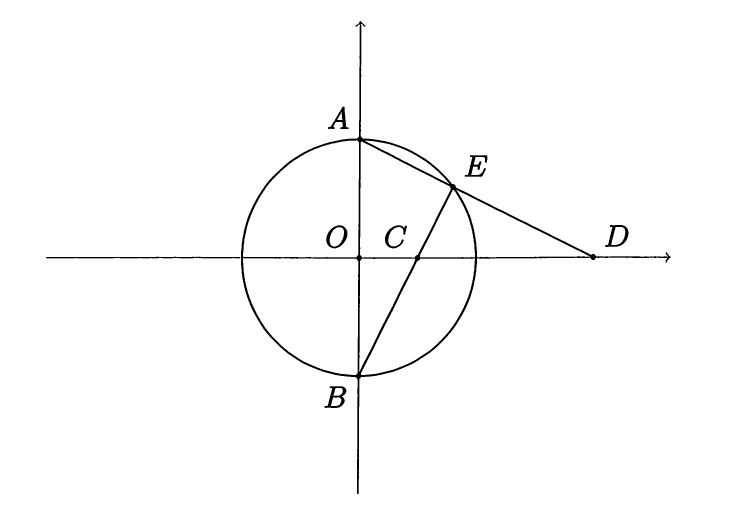
\includegraphics[scale=.25]{stereo.png}
		\caption{The triangles \(OBC\) and \(ODA\) are similar so \(|OC||OA|=1\)}
	\end{figure}
\end{frame}

\begin{frame}{The Riemann sphere \(\CP^1 \cong S^2\)}
	Inversion in the unit circle
	\[
	S^1 \subset \R^2 \cong \C
	\]
	is given by 
	\[
	\xi \mapsto \bar{\xi}^{-1}
	\]
	Composing one of the \(2\) stereographic projections with complex conjugation identifies \(S^2\) with two copies of \(\C\) glued by \(\xi \mapsto 1 /\xi\)
	\[
	S^2 \cong \CP^1
	\]
	Under this identification \(H: S^3 \to \CP^1\) is the Hopf map
	\[
	H(z, w) = (|z|^2 - |w|^2, z \bar{w})
	\]
\end{frame}

\begin{frame}{Fibres}
	\(S^3\) is the union of two solid tori 
	\[T_1 = \{|z|^2 \leq 1/2\}\, \text{ and } \, T_2 = \{|w|^2 \leq 1/2\}\] 
	glued along the Clifford torus \(|z|=|w|=1/\sqrt{2}\)
	\pause
	\begin{figure}
		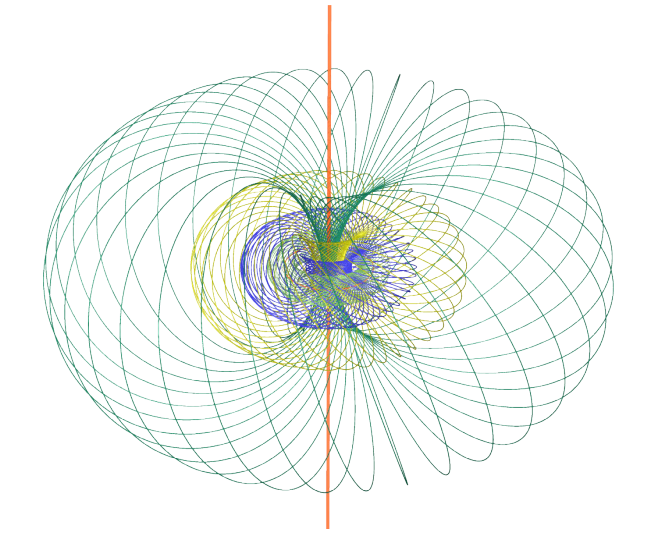
\includegraphics[scale=.25]{fibration.png}
		\caption{The intersection of the coordinate lines with \(S^3\) are the core circles of \(T_1\) and \(T_2\). The diagonal \(z=w\) intersects \(S^3\) along a \((1,1)\) circle lying on the Clifford torus.}
	\end{figure}
\end{frame}

\end{document}
